\documentclass[12pt, a4paper]{article}
\usepackage[francais]{babel}
\usepackage{caption}
\usepackage{pgfplots}
\usepackage{graphicx}
\usepackage[T1]{fontenc}
\usepackage{listings}
\usepackage{geometry}
\usepackage{tikz}
\usepackage{pgfplots}
\usepackage{amsmath}
\usepackage{minted}
\usepackage{array,multirow,makecell}
\usepackage[colorlinks=true,linkcolor=black,anchorcolor=black,citecolor=black,filecolor=black,menucolor=black,runcolor=black,urlcolor=black]{hyperref}
\setcellgapes{1pt}
\makegapedcells
\usepackage{fancyhdr}
\pagestyle{fancy}
\lhead{}
\rhead{}
\chead{}
\rfoot{\thepage}
\lfoot{Martin Baumgaertner}
\cfoot{}
\pgfplotsset{compat=1.11}
\renewcommand{\footrulewidth}{0.4pt}
\renewcommand{\headrulewidth}{0.4pt}
\renewcommand{\listingscaption}{Code}
\renewcommand{\listoflistingscaption}{Table des codes}
% \usepackage{mathpazo} --> Police à utiliser lors de rapports plus sérieux

\begin{document}
\begin{titlepage}
	\newcommand{\HRule}{\rule{\linewidth}{0.5mm}} 
	\center 
	\textsc{\LARGE iut de colmar}\\[6.5cm] 
	\textsc{\Large R314}\\[0.5cm] 
	\textsc{\large Année 2022-23}\\[0.5cm]
	\HRule\\[0.75cm]
	{\huge\bfseries Analyse de Fourier}\\[0.4cm]
	\HRule\\[1.5cm]
	\textsc{\large martin baumgaertner}\\[6.5cm] 

	\vfill\vfill\vfill
	{\large\today} 
	\vfill
\end{titlepage}
\newpage
\tableofcontents
\newpage
\section{CM 1 - 21 septembre 2022}
\subsection{Définition}
Un signal est dit périodique lorsque que nous pouvons retrouver un travers
un signal un zone répétée.\\
La fréquence d'un signal peut se calculer avec : $ \nu $ = $ f = \frac{1}{T} $\\[1cm]
$ f(t) $ = signal périodique de période T. Et, on l'écrira de cette manière :\\[0.5cm]
$ f(t) = a_{0} + \sum_{n=1}^{+\infty} a_{n}cos(n \omega t) + b_{n}sin(n \omega t) $\\

Les différents harmoniques de rang n peut s'écrire :\\
$ a_{n} cos(n \omega t) + b_{n}sin(n \omega t) = hn(t)$\\

Le calcul des coefficients de Fourier  :\\
$ a_{0} = \frac{1}{T} \int_{\bigtriangleup } f(t) dt $ = valeur moyenne \\[0.5cm]

Ces deux formules servent car nous pouvons calculer les données $ a_{n} $ et $ b_{n} $ 
pour la grosse formule au dessus avec le petit 1 : 
\begin{itemize}
    \item $ a_{n} = \frac{2}{T} \int_{\bigtriangleup } f(t) cos(n \omega t) dt $
    \item $ b_{n} = \frac{2}{T} \int_{\bigtriangleup } f(t) sin(n \omega t) dt $
\end{itemize}

\subsection{Exemple}

Soit le signal :\\

$ f(t) = \left\{
          \begin{array}{ll}
            1 $ si $ - \pi \leq t \leq 0 \\
            2 $ si $ 0 \leq t \leq \pi \\
          \end{array}
        \right.$

\subsubsection{Tracer le signal}
\begin{figure}[H]
    \centering
    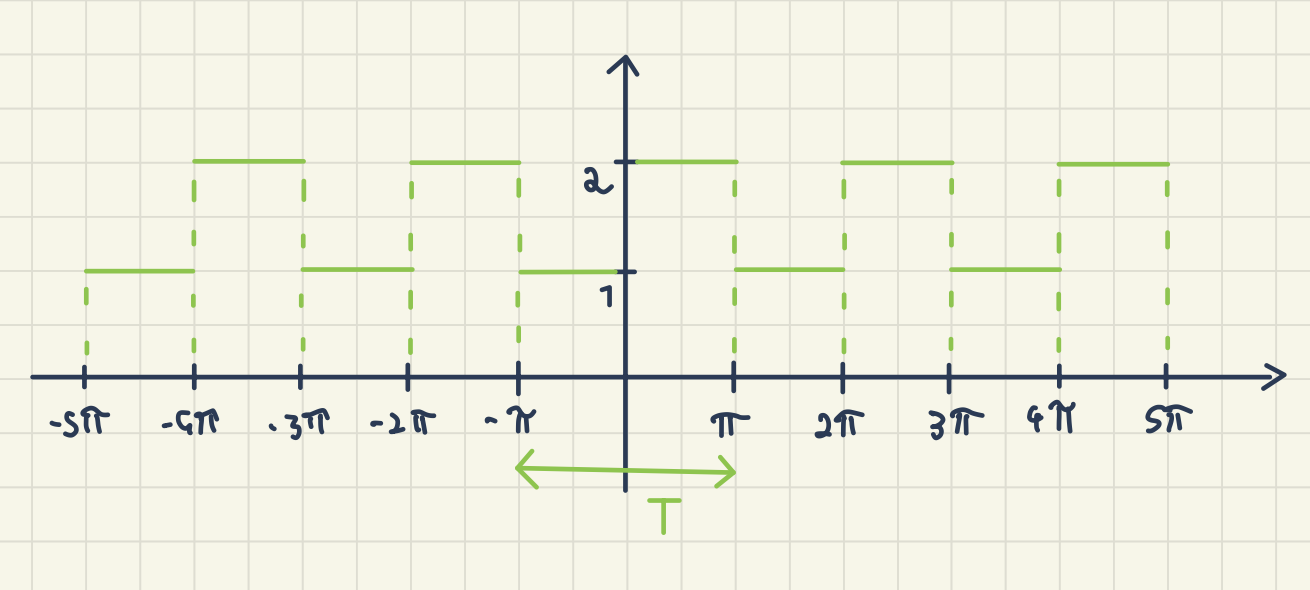
\includegraphics[width=0.9\textwidth]{img/courbe1.png}
    \caption{La courbe 1}
    \label{fig:courbe}
\end{figure}

\subsubsection{Calcul de sa valeur moyenne}

On calcule d'abord $ a_{O} = \frac{1}{T} \int_{\bigtriangleup}f(t) dt$ :\\[0.5cm]
\par $ \Rightarrow $ $ T = 2\pi $\\
\par $ \Rightarrow $ $ \bigtriangleup = [- \pi; \pi] $\\
\par $ \Rightarrow $ $ a_{0} = \frac{1}{2 \pi} \int_{- \pi}^{\pi} f(t)dt = \frac{1}{2T}(\int_{- \pi}^{0} 1dt + \int_{0}^{\pi}2dt $\\
\par $ \Rightarrow $ $ a_{0} = \frac{1}{2\pi}([t]_{- \pi}^{0} + [2t]_{0}^{\pi}) $\\
\par $ \Rightarrow $ $ a_{0} = \frac{1}{2\pi}(0 - (- \pi) + (2 \pi - 0)) $\\
\par $ \Rightarrow $ $ a_{0} = \frac{1}{2\pi}(\pi + 2 \pi) = \frac{1}{2 \pi} = \frac{3}{2} $\\

\newpage
\subsubsection{Calcul des coefficients de Fourier}

Premièrement, on calcule $ a_{n} $ et $ b_{n} $ :\\

\par $ \Rightarrow $ $ \omega = \frac{2 \pi}{T} = \frac{2 \pi}{2 \pi} = 1 $\\
\par $ \Rightarrow $ $ a_{n} = \frac{2}{T} \int_{\bigtriangleup} f(t) cos (nt) dt $\\
\par $ \Rightarrow $ $ a_{n} = \frac{2}{2 \pi} \int_{- \pi}^{\pi} f(t) cos (nt) dt $\\
\par $ \Rightarrow $ $ a_{n} = \frac{1}{\pi} [ \int_{- \pi}^{0} 1 cos (nt)dt +  \int_{0}^{\pi} 2 cos(nt)dt ] $\\
\par $ \Rightarrow $ $ a_{n} = \frac{1}{\pi}([\frac{sin(nt)}{n}]_{- \pi}^{0} + [\frac{2sin(nt)}{n}]_{0}^{\pi}) $\\ 
\par $ \Rightarrow $ $ a_{n} = 0 $\\[0.5cm]

\begin{tikzpicture}
    \begin{axis}
      [
        xtick={-7.0686,-6.2831,...,7.0686},
        xticklabels={
          ,
          {\tiny$-8\pi$},
          {\tiny$-7\pi$},
          {\tiny$-6\pi$},
          {\tiny$-5\pi$},
          {\tiny$-4\pi$},
          {\tiny$-3\pi$},
          {\tiny$-2\pi$},
          {\tiny$-1\pi$},
          {\tiny$0\pi$},
          {\tiny$1\pi$},
          {\tiny$2\pi$},
          {\tiny$3\pi$},
          {\tiny$4\pi$},
          {\tiny$5\pi$},
          {\tiny$6\pi$},
          {\tiny$7\pi$},
          {\tiny$8\pi$},
          },
        grid=major,
        x=10mm,
        y=20mm,
        axis x line=center,
        axis y line=center,
        xlabel={$x$},
        ylabel={$y$},
        every tick label/.style={fill=white},
      ]
    \addplot
      [
        domain=-2*pi:2*pi,
        smooth,
        blue,
        thick,
      ]
      plot {sin(deg(x))};
    \end{axis}
  \end{tikzpicture}\\
  La fonction sinus est impaire car $ f(-x) = -f(x) $\\
\subsubsection{Donner sa décomposition en série de Fourier}

\subsubsection{Donner les 4 premières harmoniques}

\subsubsection{Trucs et astuces}

\begin{itemize}
    \item Si $ f(t) $ est pair alors les $ b_{n} $ sont nuls
    \item Si $ f(t) $ est impair alors $ a_{0} $ les $ a_{n} $ sont nuls
    \item Si $ f(t) $ est quelconque mais que $ f(t) - a_{O} $ est impair alors les
    $ a_{n} $ sont nuls 
\end{itemize}

\newpage

\section{CM 2 - 13 janvier 2023}
\subsection{Intégrales}
\par $ \Rightarrow \int_{- \pi}^{\pi}  sin(2t)dt $\\

La primitive de $ sin(t) $ est $ -cos(t) $\\

Sauf que dans notre cas ça ne s'applique pas, il va donc falloir revenir sur le
sinus d'une variable :

on pose $ u = 2t $ \\
\par $ du = u' dt $ \\
\par $ du = 2t $ \\
\par $ \frac{du}{2} = dt $ \\
\par $ I = \int sin(u)\frac{du}{2} = \frac{1}{2}\int sin(u) du $ \\
\par $ \frac{1}{2} [-cos(u)] = \frac{1}{2}[-cos(2t)]_{-\pi}^{\pi} = [\frac{-cos(2t)}{2}]_{-\pi}^{\pi} = 0 $ \\  

L'intégral d'une fonction impaire sur l'intervalle symétrique par rapport à 0 est nulle.\\



\end{document}